\documentclass[10pt,a4paper]{article}
\usepackage[latin1]{inputenc}
\usepackage[T1]{fontenc}
\usepackage[french]{babel}
\usepackage{fancyhdr}
\usepackage{graphicx}
\pagestyle{fancy}

\renewcommand{\headrulewidth}{1pt}
\fancyhead[C]{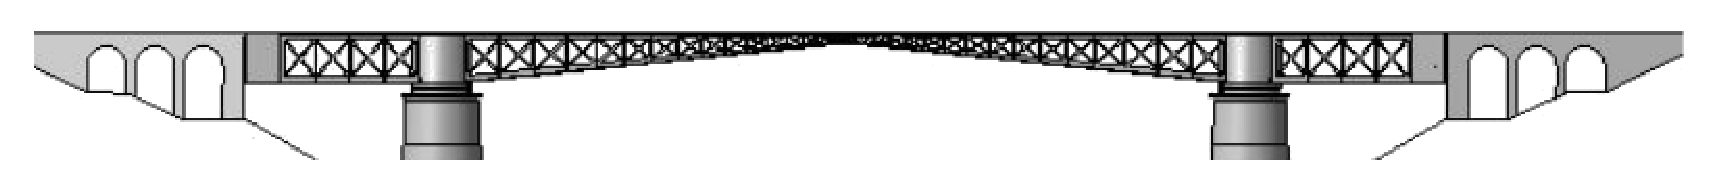
\includegraphics[width=7cm]{../images/top}}
\fancyhead[L]{
\includegraphics[width=2cm]{../images/enib}}
\fancyhead[R]{S6A-02}

\renewcommand{\footrulewidth}{1pt}
%\fancyfoot[L]{\textbf{page \thepage}}
\fancyfoot[C]{Corentin Pouplard - Fidel Nguyen - Simon Tarti�re -
  Yoann Diqu�lou}
%\fancyfoot[R]{\leftmark}

\title{{\Huge \bf R�sum� cours 03/10/2014}\\
  \vspace{0.5cm}
\centerline{  Corentin Pouplard - Fidel Nguyen}
\centerline{ Simon Tarti�re -  Yoann Diqu�lou}
\vspace{0.5cm}
\date{\today}
}
\begin{document}
\maketitle
\thispagestyle{fancy}
\hrule
\section*{Objectif}
Pr�parer les diagrammes UML
\section*{Travail effectu�}
Lors de cette s�ance, nous avons �num�r� un ensemble de
fonctionnalit�s li�es aux syst�mes:

\section*{Actions}
Mise en mouvement du pont: 
\begin{itemize}
\item Rentrer les verrous
\item Ouvrir les machoires
\item Actionner les cabestants
\end{itemize}

Fermeture:
\begin{itemize}
\item    fermer les machoires
\item    fermer les verrous
\end{itemize}

\section*{Actions de l'acteur}
Les diff�rentes actions que nous avons identifi�es sont:
\begin{itemize}
\item Se d�placer
\item Int�ragir avec les diff�rents m�canismes
\item Changer la force applicable sur les cabestants
\end{itemize}

\section*{Syst�mes globaux identifi�s}
Nous avons identifi�s 4 syst�mes globaux, eux-m�me constitu� de
sous-syst�me (que nous d�taillerons plus tard):
\begin{itemize}
\item Verrous
\item Machoires
\item Cabestants et engrenages
\item Trav�es
\end{itemize}

\section*{Id�es abord�es}
Nous avons abord� l'id�e que l'utilisateur puisse se d�placer
librement, puis lorsqu'il actionne un syst�me, on d�place la cam�ra
sur ce syst�me, puis � partir de ce moment, il peut continuer � ce
d�placer librement.

\section*{A faire rapidement}
Prendre contact avec Pierre Vanderwagen pour r�cup�rer les plans du
pont.\\
D�buter les diagrammes UML.
\end{document}
